% UTF-8 encoding
% Compile with latex+dvipdfmx, pdflatex, xelatex or lualatex

\documentclass[hyperref, UTF8]{ctexart}
\usepackage{graphicx}
\usepackage{amssymb}
\usepackage{amsmath}
\usepackage{subfigure}
\usepackage{geometry}
\usepackage{caption}
\usepackage{upgreek}
\newcommand{\volt}{{\rm V}}
\newcommand{\source}{{\rm S}}
\newcommand{\ampere}{{\rm A}}
\newcommand{\hertz}{{\rm Hz}}
\newcommand{\ohm}{\Omega}
\newcommand{\kiloohm}{{\rm k}\Omega}
\newcommand{\watt}{{\rm W}}
\newcommand{\kilowatt}{{\rm kW}}
\newcommand{\degree}{^{\circ}}
\newcommand{\farad}{{\rm F}}
\newcommand{\microfarad}{{\rm \upmu F}}
\newcommand{\millifarad}{{\rm mF}}
\newcommand{\henry}{{\rm H}}
\newcommand{\J}{{\rm j}}

\title{电子学基础——第一次仿真作业}
\author{LXQ}
\date{2019.10.17}

\geometry{left=2.0cm, right=2.0cm, top=2.5cm, bottom=2.5cm}
\linespread{1}

\begin{document}

\maketitle

\paragraph{A-1}
利用合适的仿真方法,求题图 A-1 中每个电路的等效电路。

\begin{figure}[!htb]
\centering
\begin{minipage}[t]{0.389\textwidth}
\centering
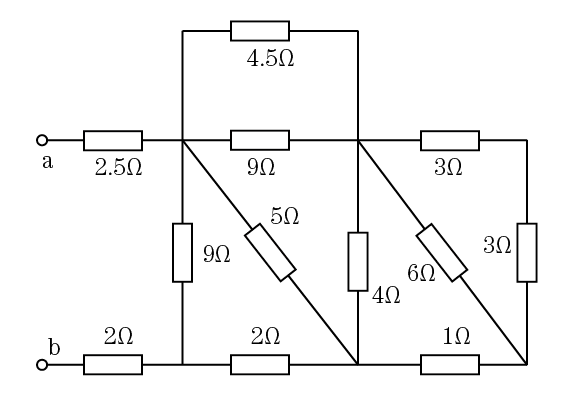
\includegraphics[width=1\textwidth]{pA-1-a.png}
\caption*{(a)}
\end{minipage}
\begin{minipage}[t]{0.333\textwidth}
\centering
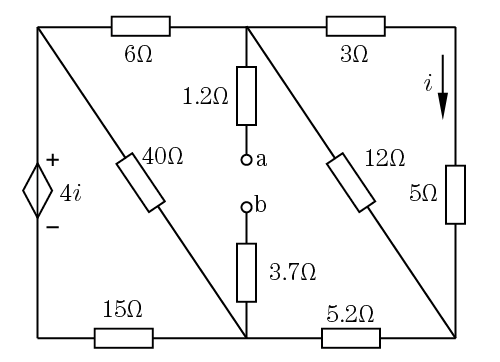
\includegraphics[width=1\textwidth]{pA-1-b.png}
\caption*{(b)}
\end{minipage}
\caption*{题图 A-1}
\end{figure}

\paragraph{答}
(a) 如图 A-1-(a) 所示,$ab$两端接$10 \volt$电压,通过电流为$1.33 \ampere$,而整个电路仅含电阻,则电路可简化为$75\ohm$电阻。\\

(b) 如图 A-1-(b) 所示,$ab$两端接$10 \volt$电压,通过电流为$0.861 \ampere$,而整个电路仅含电阻和受控电源,则电路可简化为$11.61\ohm$电阻。

\begin{figure}[!htb]
\centering
\begin{minipage}[t]{0.359\textwidth}
\centering
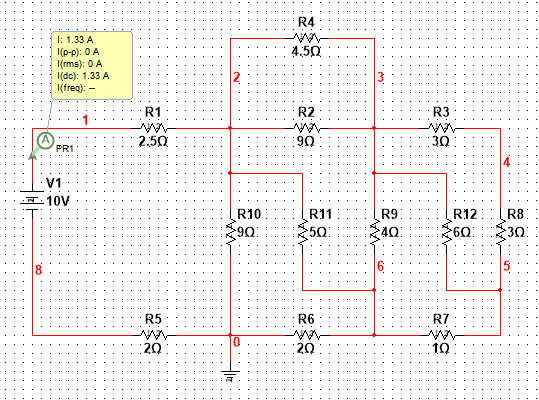
\includegraphics[width=1\textwidth]{pA-1-a-sim.png}
\caption*{(a)}
\end{minipage}
\begin{minipage}[t]{0.425\textwidth}
\centering
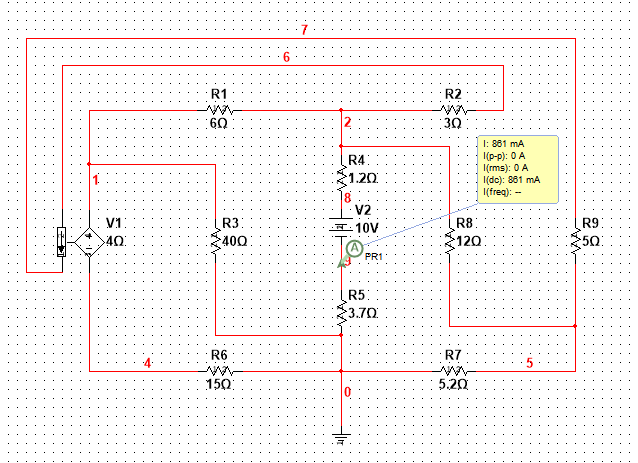
\includegraphics[width=1\textwidth]{pA-1-b-sim.png}
\caption*{(b)}
\end{minipage}
\caption*{图 A-1}
\end{figure}

\paragraph{A-4} 电路如图 A-4 所示,已知电压信号$u_0 = 10 + 10 \sin 2000 \pi t \volt $。试同时观察信号源和电容上的电压波形,比较两者的区别,并说明原因。

\begin{figure}[!htb]
\centering
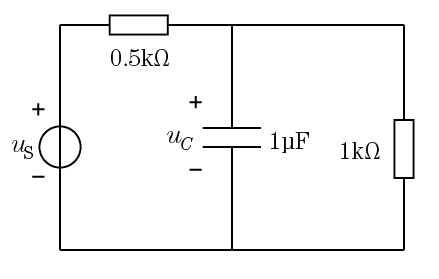
\includegraphics[width=0.293\textwidth]{pA-4.png}
\caption*{题图 A-4}
\end{figure}

\paragraph{答} 仿真电路和示波器结果如图 A-4 所示。示波器中蓝色曲线为电源电压,绿色曲线为电容上的电压。比较可知:(1) 两个电压均在正值以上波动,这是电源电压中直流分量导致的结果;(2) 电容上电压的波动峰值小于电源电压波动峰值,这是由于干路上电阻分压;(3) 电容上电压波峰要滞后于电源电压波峰,这是由于电容的电抗为 $X_C<0$ 所导致的结果。

\begin{figure}[!htb]
\centering
\begin{minipage}[t]{0.354\textwidth}
\centering
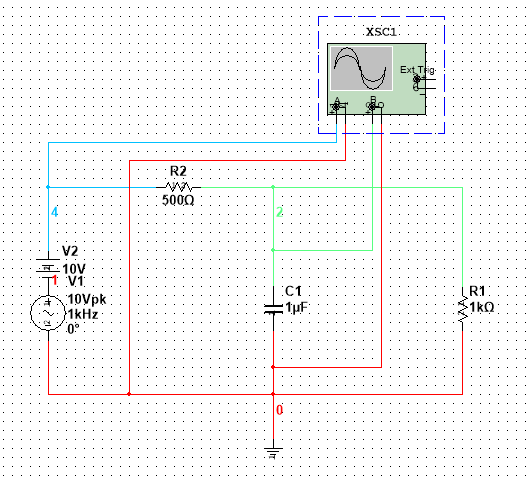
\includegraphics[width=1\textwidth]{pA-4-sim.png}
\caption*{(Simulation)}
\end{minipage}
\begin{minipage}[t]{0.550\textwidth}
\centering
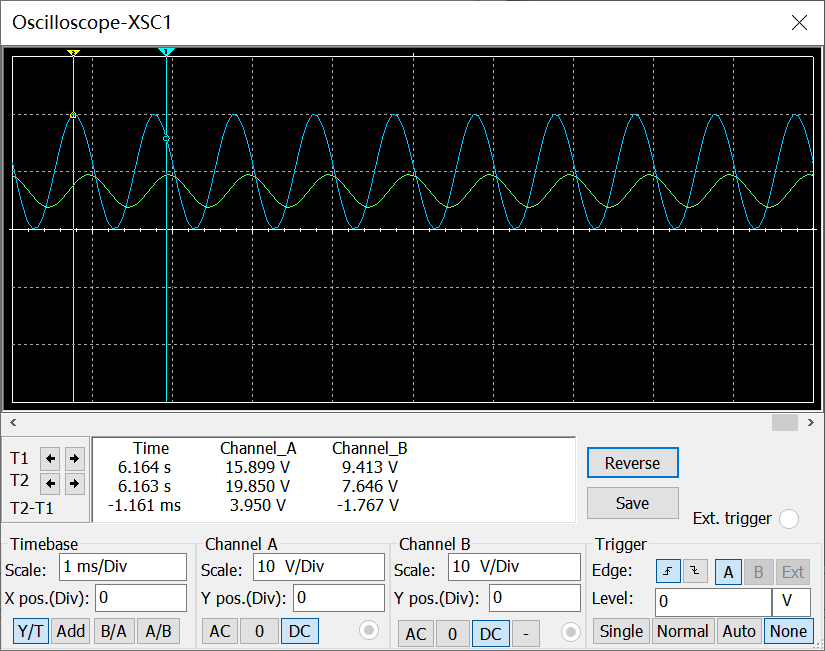
\includegraphics[width=1\textwidth]{pA-4-res.png}
\caption*{(Result)}
\end{minipage}
\caption*{图 A-4}
\end{figure}


\end{document} 